\documentclass[12pt,a4paper]{article}
\usepackage[utf8]{inputenc}
\usepackage{enumitem}
\usepackage{geometry}
\usepackage{graphicx}
\usepackage{textcomp}
\usepackage{hyperref}
\usepackage{xcolor}
\newlist{steps}{enumerate}{1}
\setlist[steps, 1]{label = Step \arabic*:}
\urlstyle{same}

\begin{document}

\begin{titlepage}
\begin{center}
\textup{\large{\bf Indian Institute of Information Technology Allahabad} \\ Department of Information Technology}\\[0.2in]
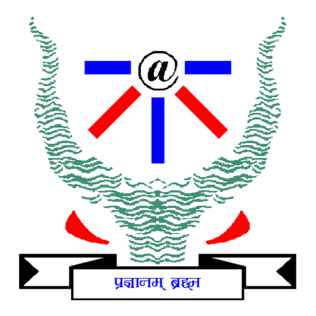
\includegraphics[width=0.35\textwidth]{./pictures/iiita_logo.png}\\[0.25in]
% Title
\Large \textbf {Image and Video Processing Course 2021}\\
       {Progress Report on \\ \bf Road Highlighting in High resolution Satellite Images}\\[0.25in]

% Submitted by
\normalsize Submitted by \\
\begin{table}[h]
\centering
\begin{tabular}{lr}
\hline \\
Roll No & Name \\
\\
\hline
\\
IIB2019002 & Pradhuman Singh Baid \\
IIB2019008 & Shyam Tayal \\
IIB2019009 & Abhijeet Sonkar \\
IIB2019010 & Avneesh Kumar \\
IIB2019013 & Arvind Uikey \\
IIB2019021 & Hitika Rajesh Kumar \\
\\
\hline
\end{tabular}
\end{table}

\vspace{.1in}
Under the guidance of\\
{\textbf{Dr. S.R. Dubey}}\\[0.1in]
\vfill
\end{center}
\end{titlepage}

 \newgeometry{
 a4paper,
 total={170mm,257mm},
 left=40mm,
 top=25mm,
 bottom=25mm,
 right=25mm
 }

\begin{abstract}
In today's growing world, there is a need for more urban planning
too high. In this paper, an efficient and effective method of extraction
of routes from the set of database provided are defined. Roads play an important
role in urban planning and therefore, its extraction is often very helpful. The Other applications for road extraction are: identification of isolated buildings
requiring the acquisition and update of the GIS dataset in accordance with
human knowledge requirements. In this way, the roads are extracted solely to
support their color. The steps within the algorithm are easy to follow and
use. It also consumes less time and is the automatic method

\end{abstract}
\bigskip

\section{Introduction}
Road highlighting plays one of the major roles in many related programs
satellite imagery. Therefore, the need to highlight the road using robust and
the effective method additionally is very high.
At the moment, there are some ways to highlight roads manually and automatically using
high-resolution satellite images. Road highlighting is described in this paper
it only depends on the color of the road. The advantage of this method is that road
images of any type of satellite are usually used as long as they are more than 0.5m
solution. Here, the imaginary images are the most spectral images. Multiple spectral
images are those images that contain three or more spectral bands. Any kind of roads
they are often extracted to support their color.
\subsection{\textbf{Motivation}}
Google maps and navigation systems are not a hundred percent accurate. Also, they don’t show the current scenario, they rely on old data. In the present scenario, they are the only options for roads detection. Sometimes due to constructions or maintenance of roads, these navigation technologies may mislead users as it does tell the current situation of roads. \\
So there is a need to overcome the inaccuracy and inconsistency problems, therefore we propose this model of road highlighting in which we are highlighting the roads using the current scenario.

\subsection{\textbf{Objective}}
As the needs and necessities are rapidly increasing in this fast developing world,it is extremely crucial at this point that their should be proper and precise planning to fulfill the necessities of urban and modern-day planning.In this report,their is an explanation to find efficient methods for highlighting the roads with the help of given databases.Roads play a very important role in modern planning and structure and so because of this reason its highlighting is of huge help.\\
There are many applications of road highlighting like in google maps or to pick out a few remoted buildings that need to be determine and updating of the geographic information system (GIS) database under the supervision of some expertise.The algorithm or set of rules is simple and handy to implement.

\subsection{\textbf{Literature Review}}
There are many works to be found in literature, however  a  handful important works
are reviewed as follows.\\
Xiangyun Hu et al. [4] introduced an automatic road centerline extraction using
high-resolution satellite images and it have gained much interest recently
in the increasing availability of high-resolution satellite images. They
propose a grouping strategy in order to automatically remove the road
center lines from high-resolution satellite images. Hierarchical collections here are
meant that instead of collecting all the segments at once, the selected segments were merged
gradually, and more indicators are integrated around the process. With this
means that the cost of the calculation can be significantly reduced.\\
With the collection of sequential steps, the segments of the separated line obtained eventually formed the long main road lines.Their proposed route has been re-tested
authorized using a few images of Ikonos and QuickBird in open spaces and construction
urban areas. The results have shown its strength and effectiveness in
extracting out the middle lines of the highway.\\
Anil et al. have once suggested that for spatial data capturing and updating of GIS applications ,road extraction from high resolution imagery is of supreme value and of great importance.He along with his team have researched and tried to make an attempt on this area i.e to  automate  the  process of extracting roads from high resolution imagery.Their project and work took help from and used  statistical region merging for image segmentation and road network has been extracted based on contour partitioning based skeleton  pruning  method,  where  the  partitions  are  obtained  by  Discrete  Curve Evolution.

\newpage
\section{Methodology}
Below are the steps that we used to extract roads from satellite images.
\subsection{Steps}
\begin{enumerate}
\item \textbf{Read Image:} This is very first and basic step in image processing. Here we our input image.
\item \textbf{Convert to Gray-scale:} This step is to transform our input image to its gray scaled form.
\item \textbf{Perform Contrast Stretching:} Before doing any image manipulations, we apply contrast stretching to image so that details in image become more clearer.
\item \textbf{Perform Thresholding:} In this step, we take certain gray level intensity value any perform thresholding. All gray levels below threshold value are set to 0 and above are set to 255(highest possible gray level).
\item  \textbf{Median Filtering:} Median Filtering is used to reduce noise from image. If, there is no noise, then there is no need to apply this filtering.
\item \textbf{Dilation:} Dilation expands the image pixels i.e. it used for expanding element A in image by using structuring element B. It adds pixels to image boundaries. It helps in recovering small of pixels happened in image.
\item \textbf{Morphological Enhancement:} This is very crucial step in complete process. Here is tend to remove small objects and regions from binary image. We provide a minimum size of region and connectivity mode and based on that we remove regions that have less pixels than minimum size. In this case we have 2 connectivity modes - a) 4 way connectivity where pixels are connected via edges; b) 8 way connectivity where pixels are connected via edges and corners.
\item \textbf{Closing:} Closing is reverse of opening. Closing is dilation followed by erosion. It is useful in filling small holes inside the foreground object and regions.
\item \textbf{Edge detection:} In this step we apply edge detection on image we processed until now. Edges are the boundary or outline of roads we extracted. We are applying 2 different types of edge detection. a) Canny Edge detection- edges are detected nicely but have thin edges; b) Morphological Gradient- have similar edges but a bit thicker in comparison to canny. We will use this to overlay in the original image.
\item \textbf{Closing:} Here we again apply closing operation to fill in the small details and connect pixels that are unconnected.
\item \textbf{Overlay extracted road and Input image:} This is the final image where we blend our input image with extracted roads in above step and save it.\textbf{}
\end{enumerate}
% \newpage
 \newgeometry{
 a4paper,
 total={170mm,257mm},
 left=25mm,
 top=25mm,
 bottom=25mm,
 right=25mm
 }
\subsection{Flowchart}
Here using flowchart we display the process in a pictorial way. We have also embedded output of each step. \href{https://colab.research.google.com/drive/1agcn__WBpbA9k0HENXSKC-bVSmDKB_De?usp=sharing}{\underline{Click here}} to see code on google colab.
\begin{figure}[!htb]
        \center{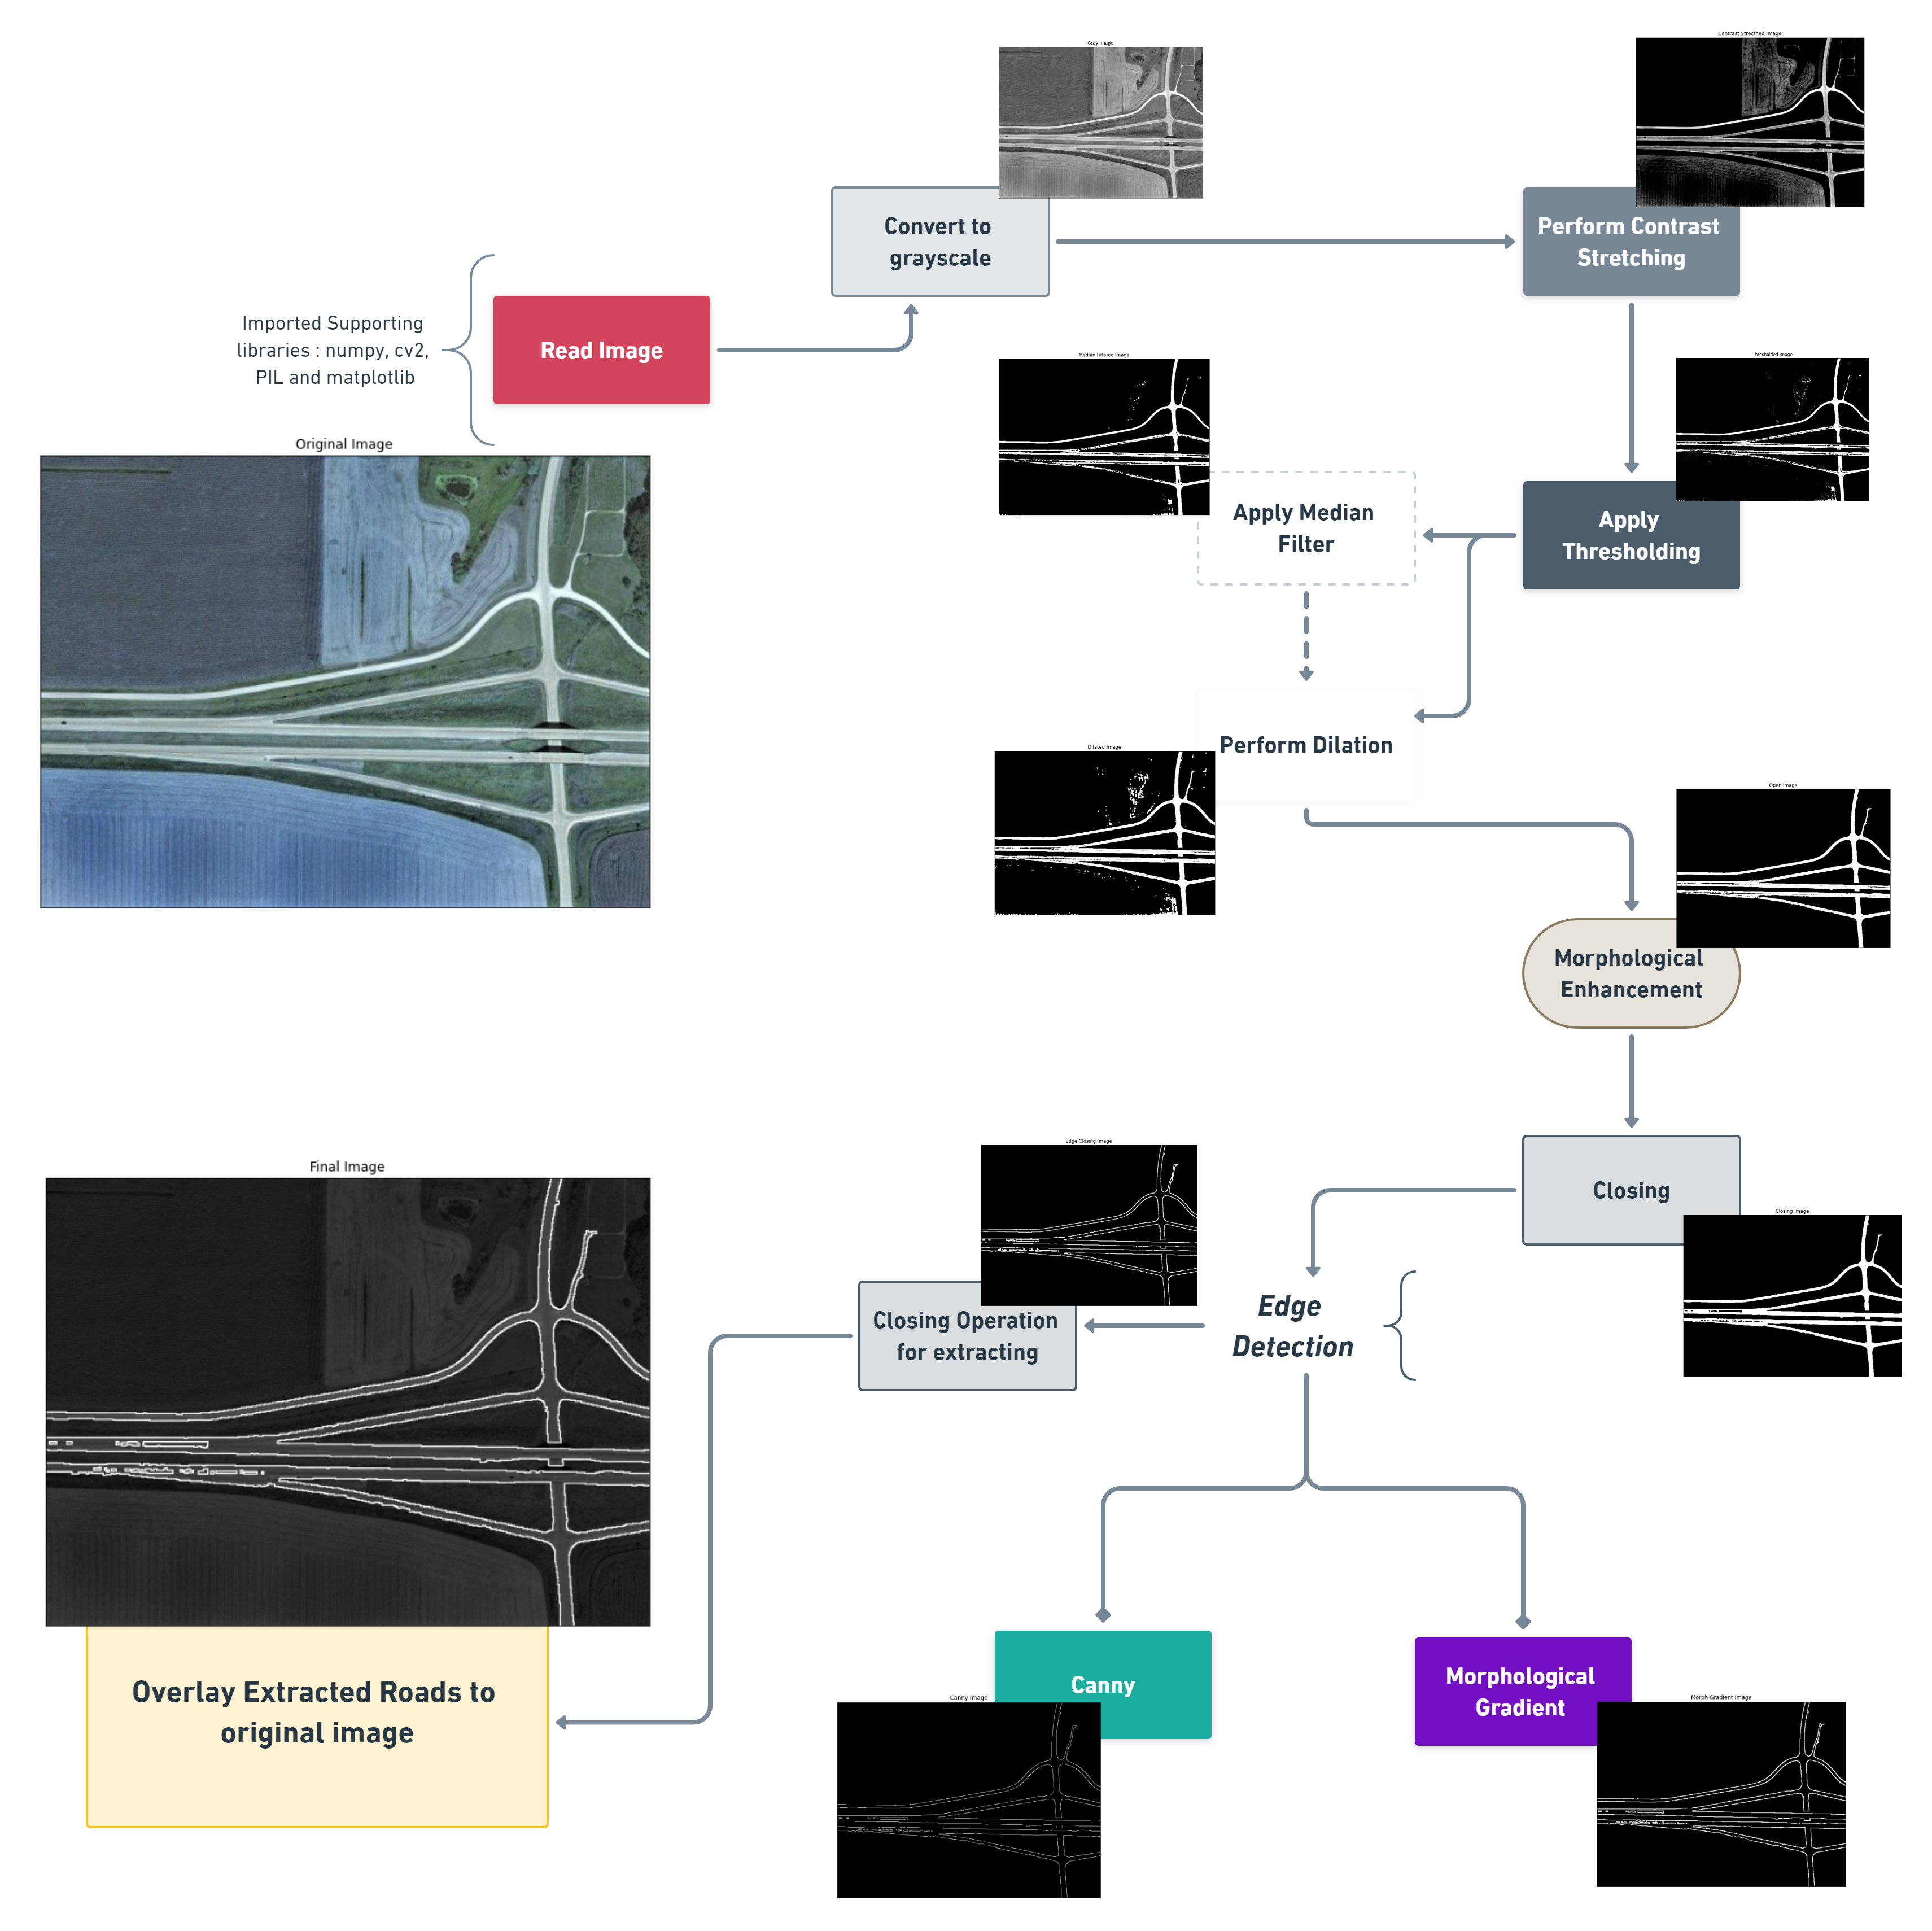
\includegraphics[width=1.1\textwidth]
        {pictures/flowchart-potrait.png}}
        \caption{\label{fig:my-label}Flowchart with stepwise output attached}
      \end{figure}

% \let\cleardoublepage\clearpage
% \newpage
 \newgeometry{
 a4paper,
 total={170mm,257mm},
 left=30mm,
 top=25mm,
 bottom=25mm,
 right=25mm
 }
\section{Dataset Images and Outputs}
\begin{tabular}{ c c c c}
 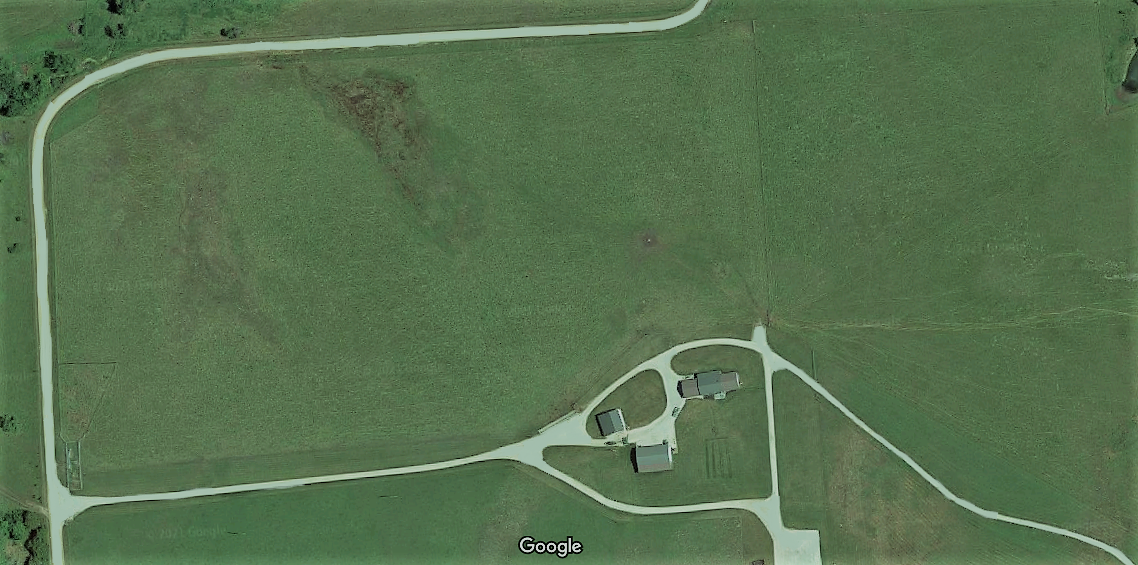
\includegraphics[width=0.25\textwidth]{./pictures/_3.png} & 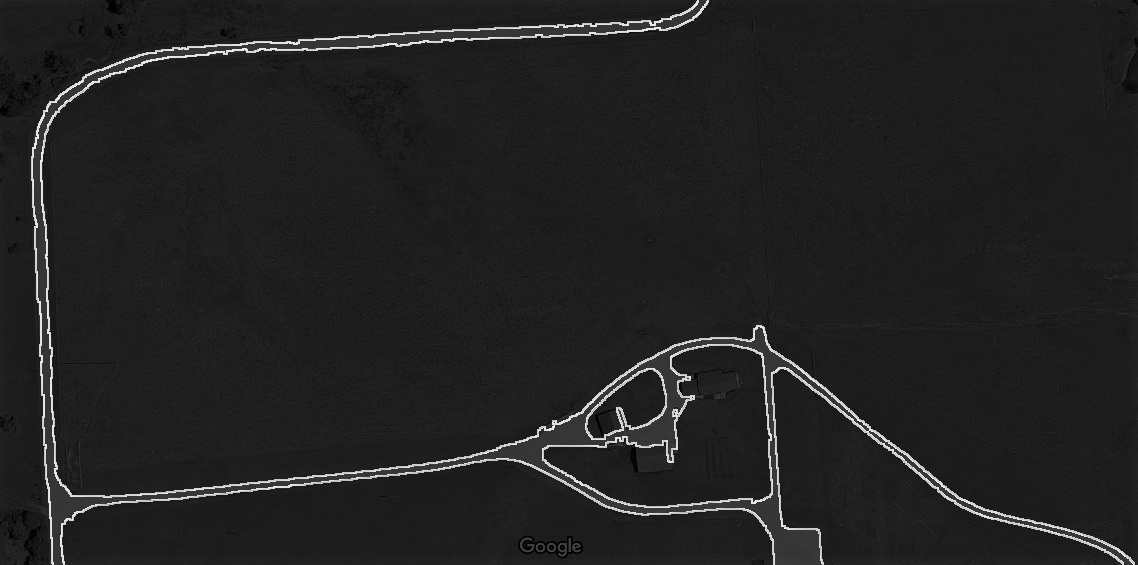
\includegraphics[width=0.25\textwidth]{./pictures/_3.png_final_img.jpg} & 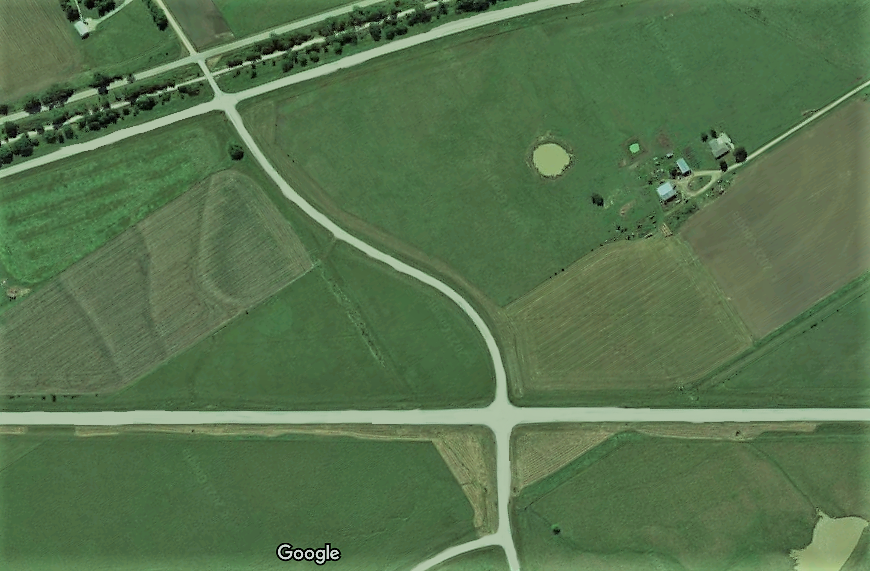
\includegraphics[width=0.25\textwidth]{./pictures/_4.png} & 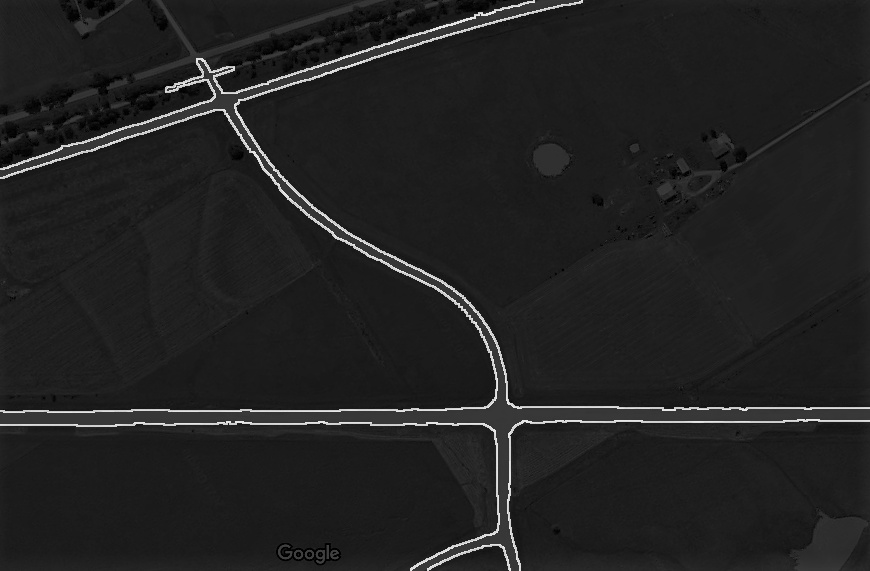
\includegraphics[width=0.25\textwidth]{./pictures/_4.png_final_img.jpg}\\
 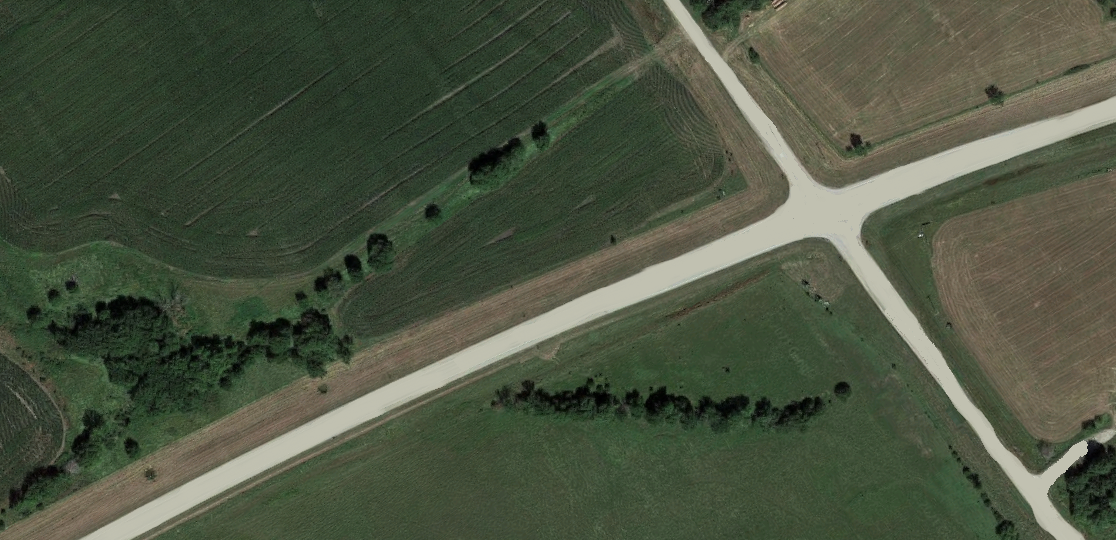
\includegraphics[width=0.25\textwidth]{./pictures/_5.png} & 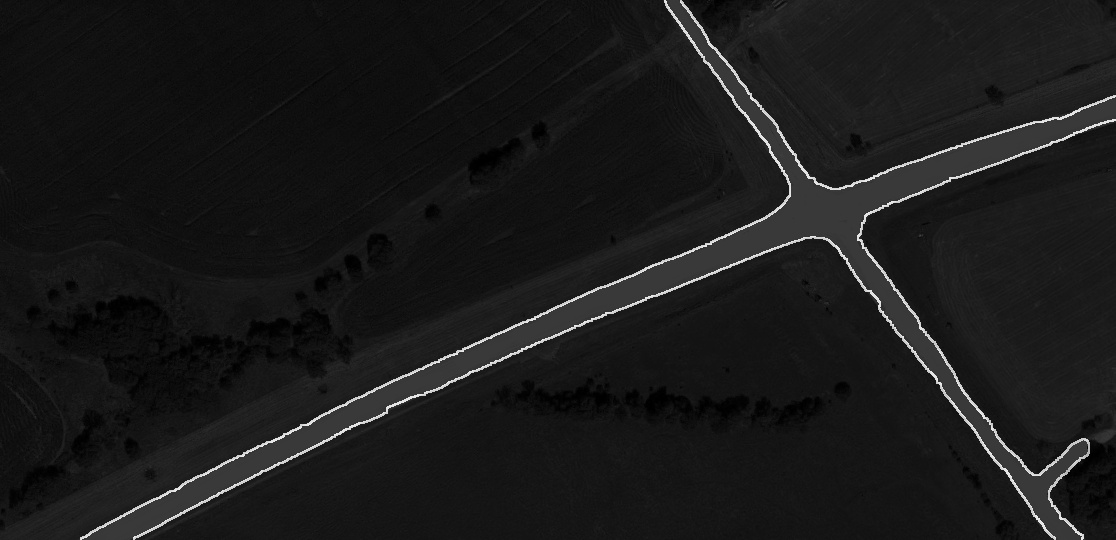
\includegraphics[width=0.25\textwidth]{./pictures/_5.png_final_img.jpg} & 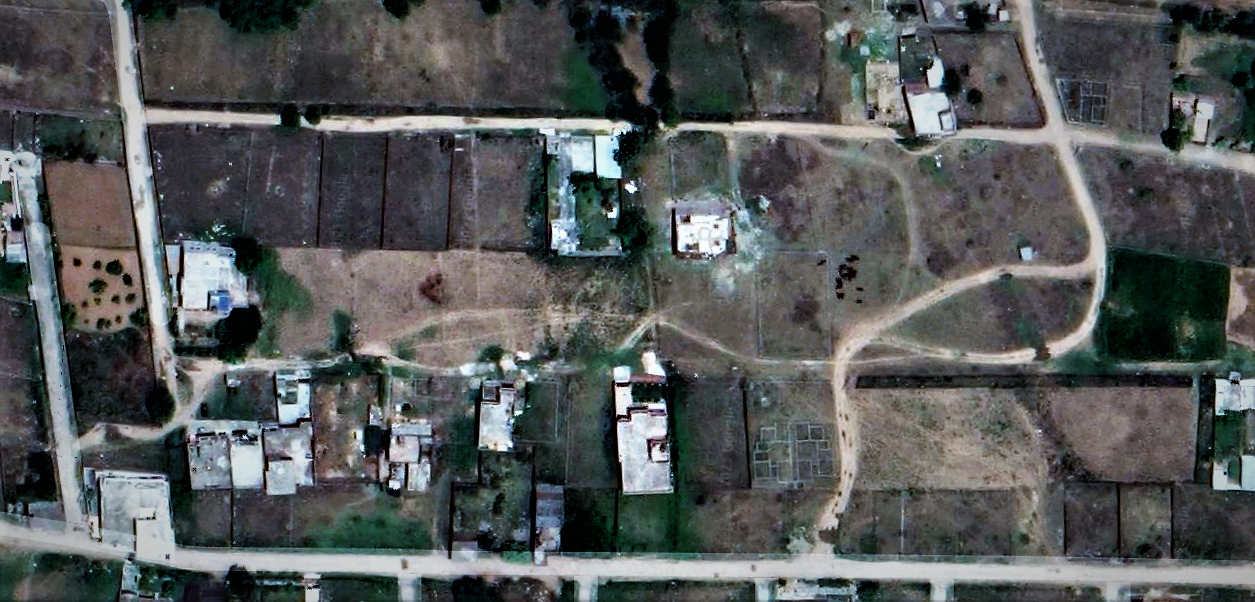
\includegraphics[width=0.25\textwidth]{./pictures/3.png} & 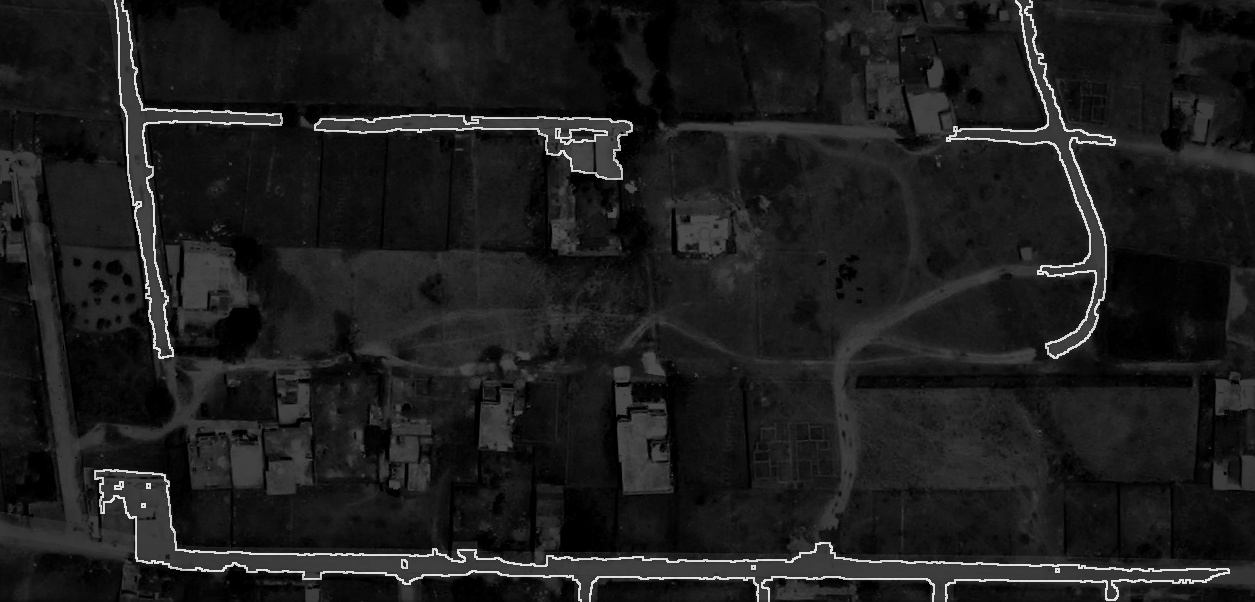
\includegraphics[width=0.25\textwidth]{./pictures/3.png_final_img.jpg}\\
 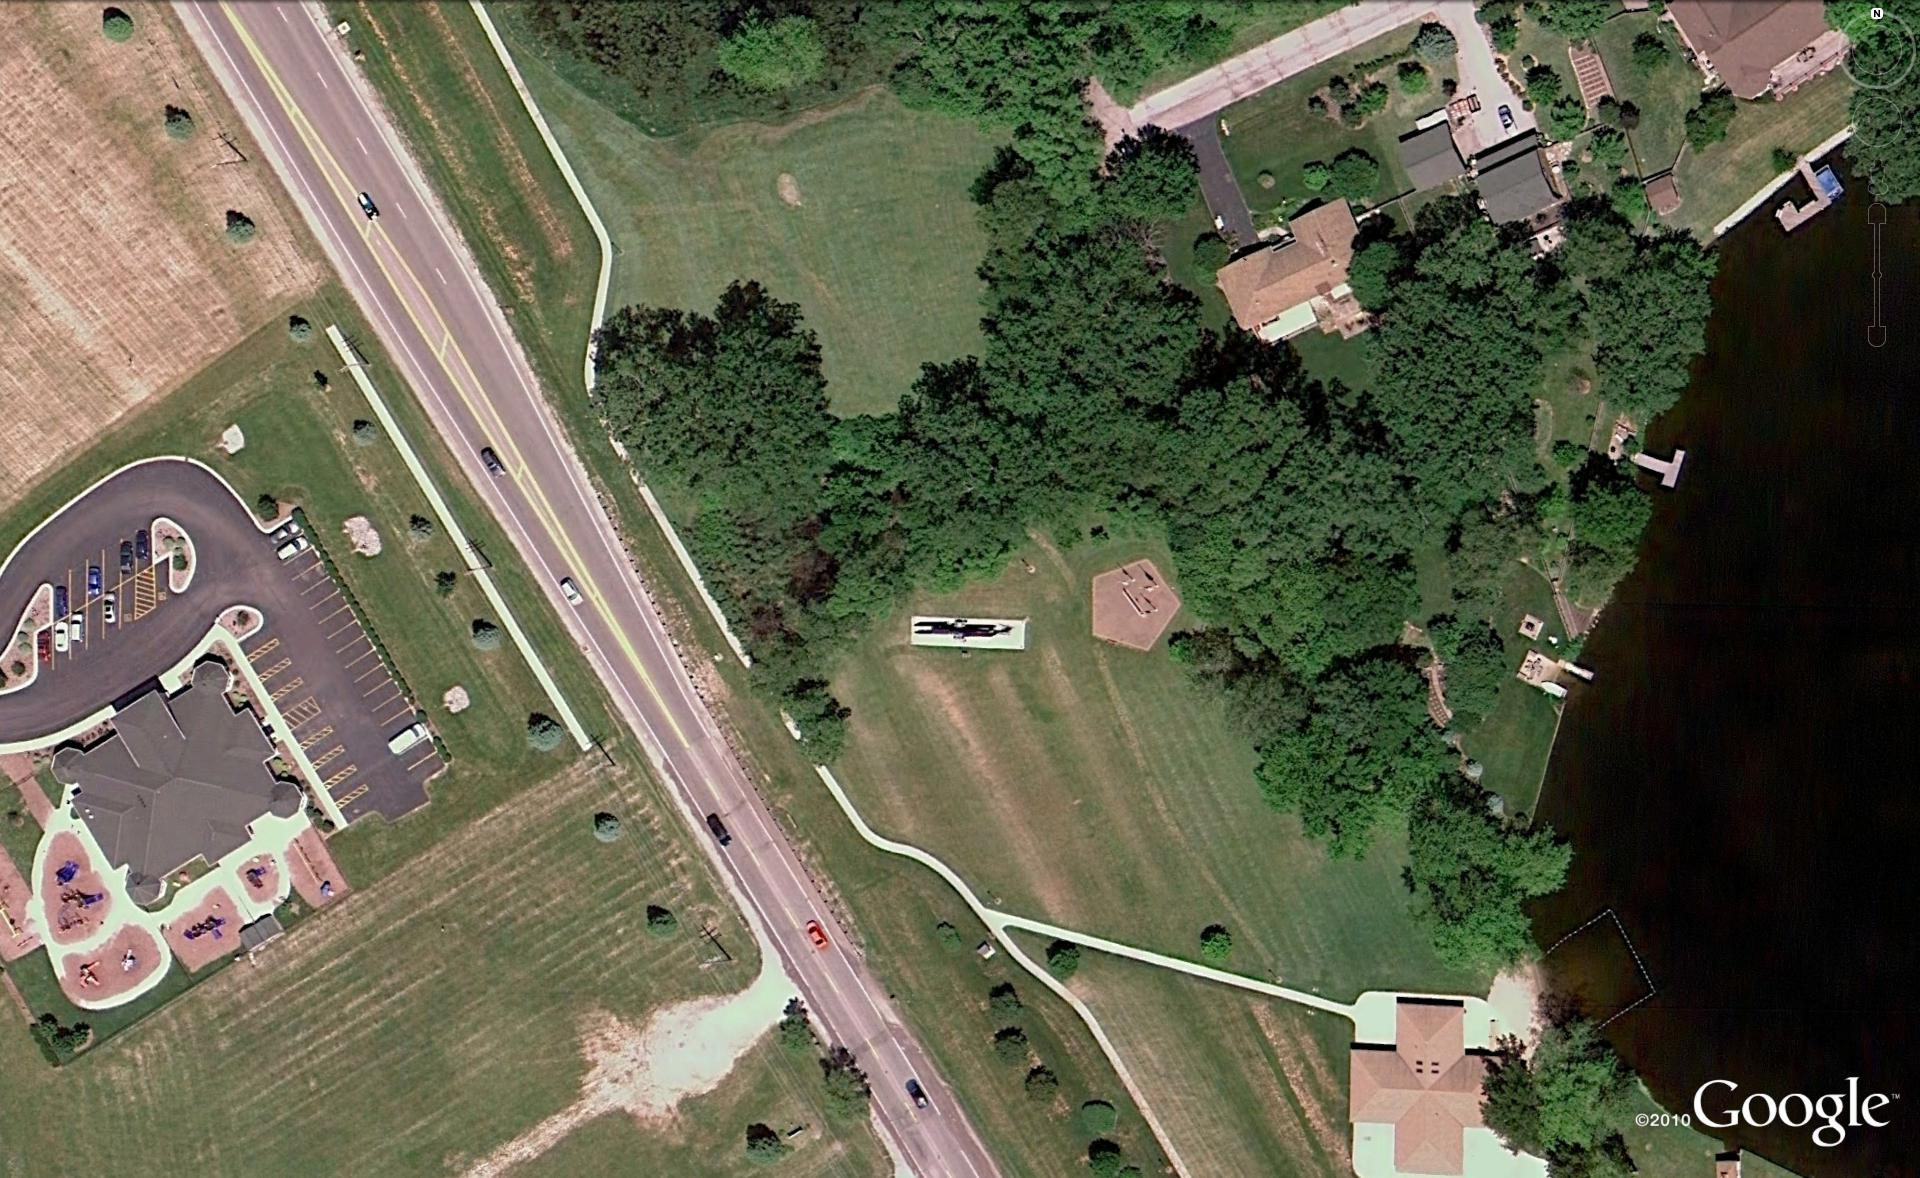
\includegraphics[width=0.25\textwidth]{./pictures/fimg2.jpg} & 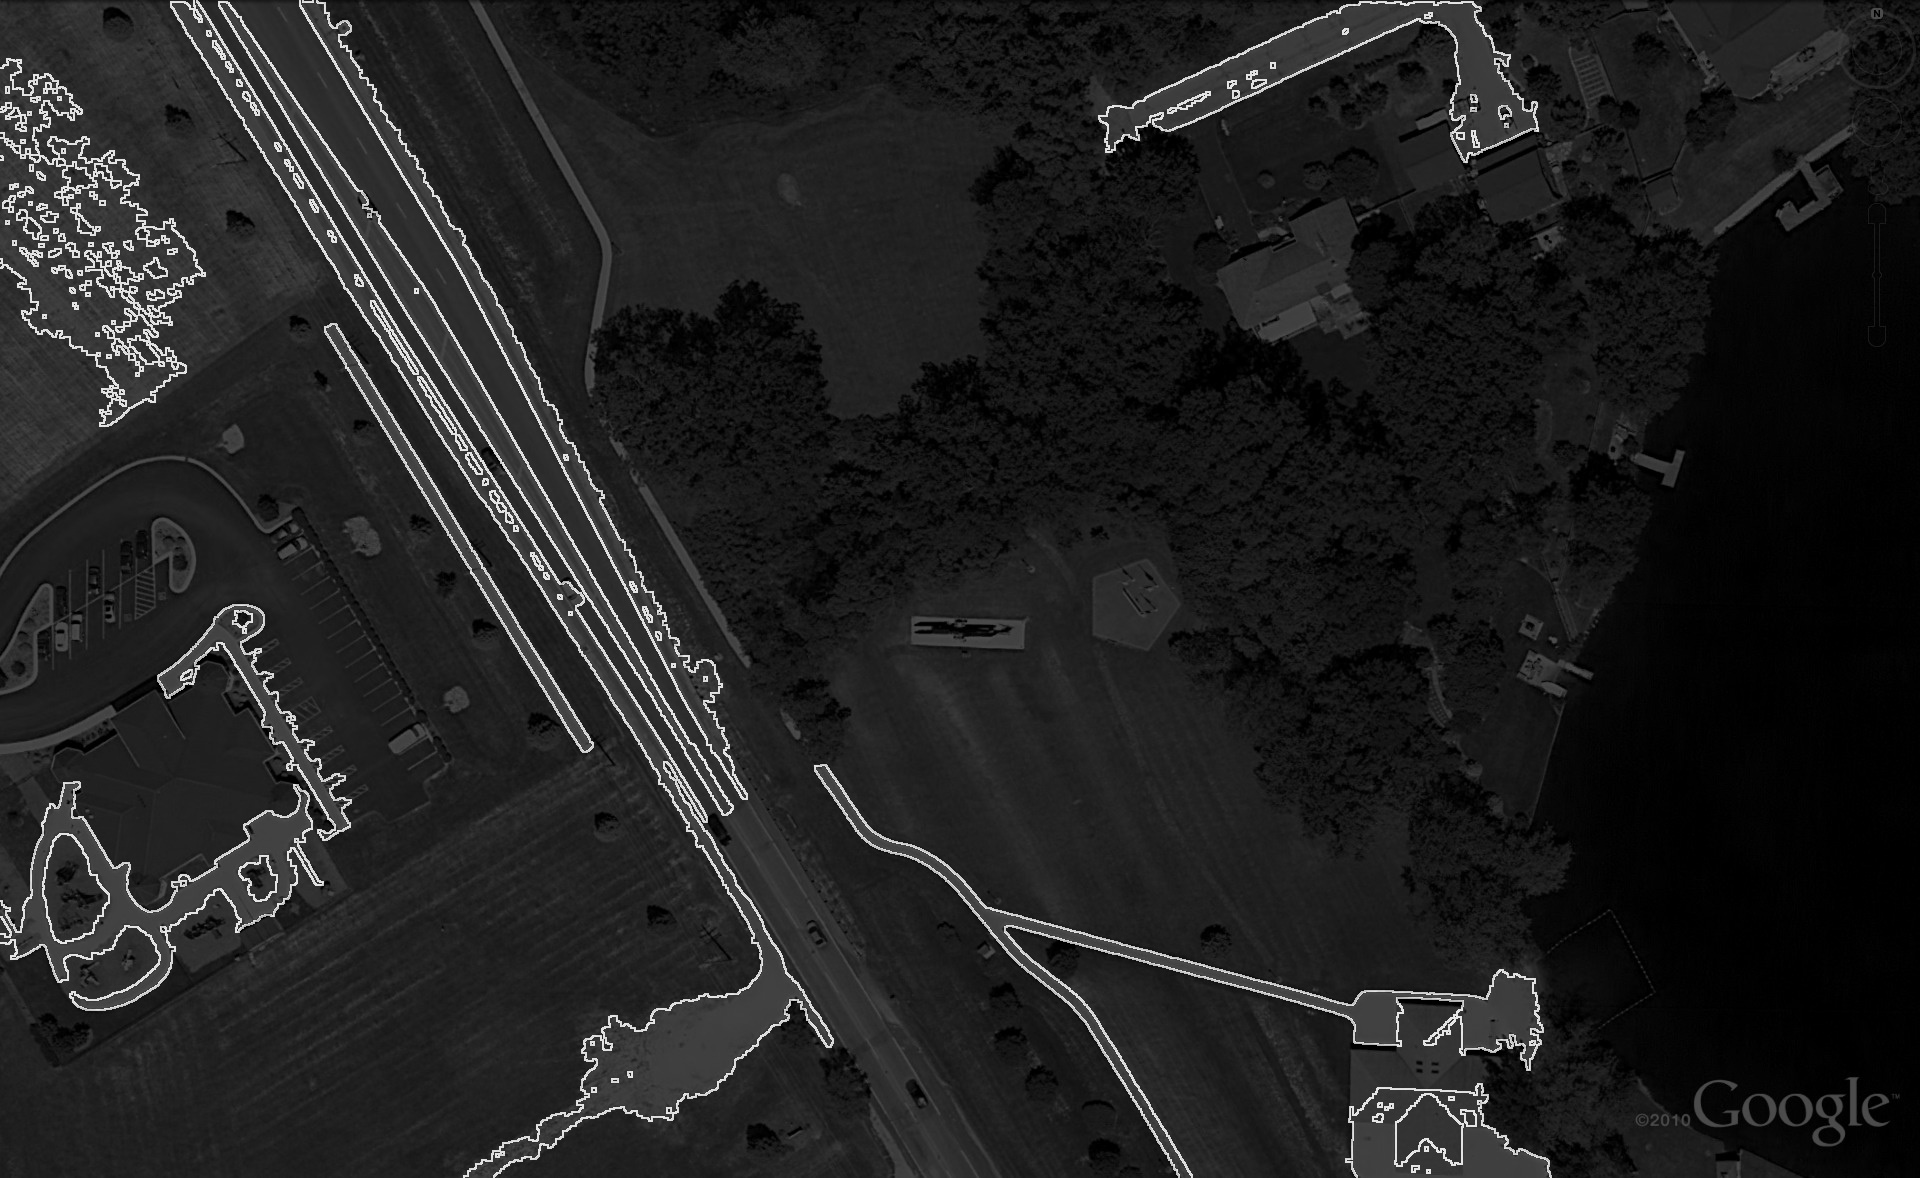
\includegraphics[width=0.25\textwidth]{./pictures/fimg2.jpg_final_img.jpg} & 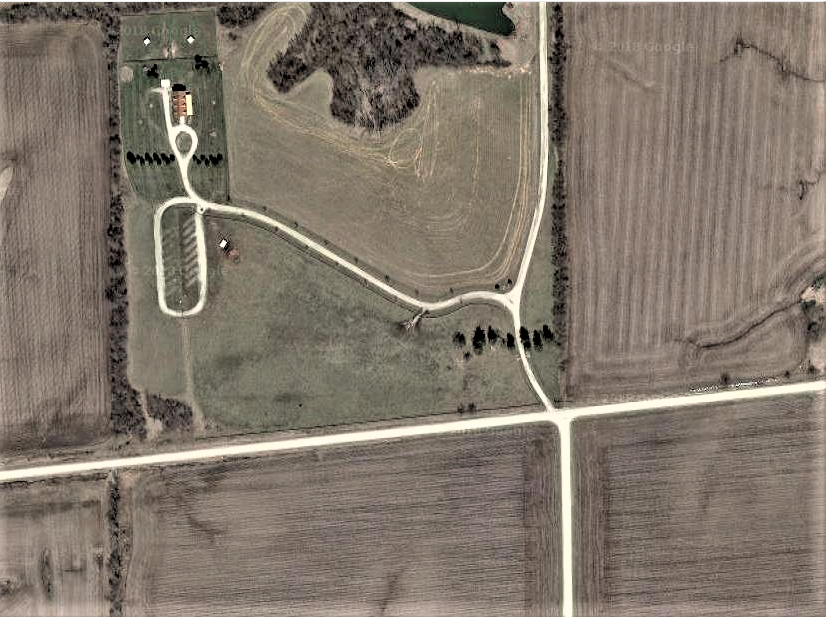
\includegraphics[width=0.25\textwidth]{./pictures/fimg3.png} & 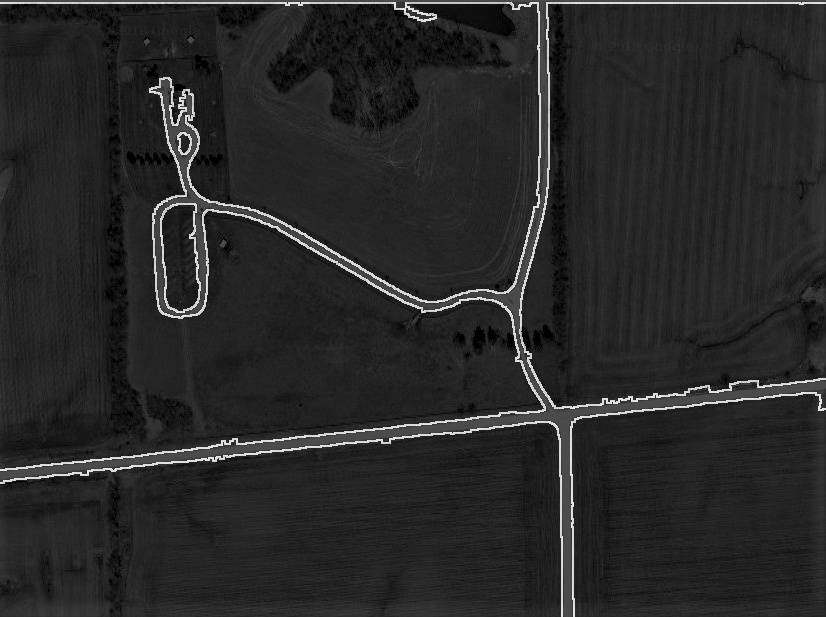
\includegraphics[width=0.25\textwidth]{./pictures/fimg3.png_final_img.jpg}\\
 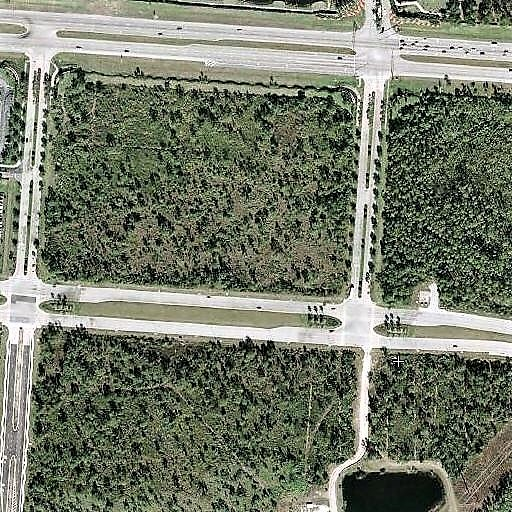
\includegraphics[width=0.25\textwidth]{./pictures/fimg4.jpg} & 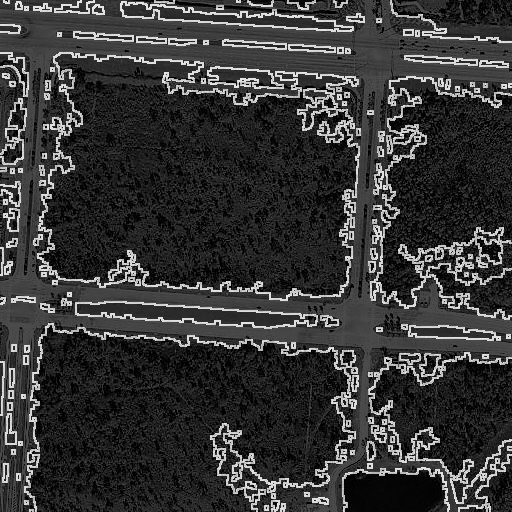
\includegraphics[width=0.25\textwidth]{./pictures/fimg4.jpg_final_img.jpg} & 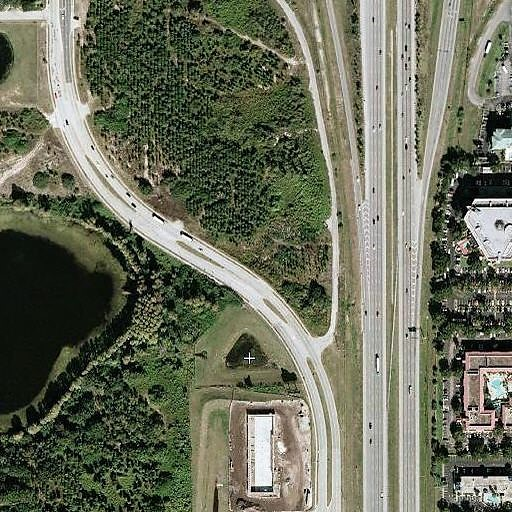
\includegraphics[width=0.25\textwidth]{./pictures/fimg5.jpg} & 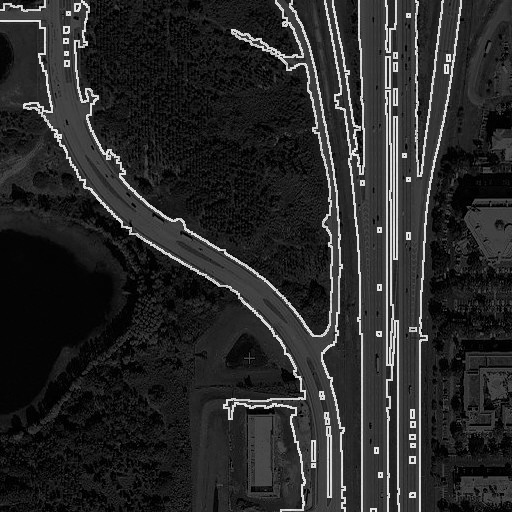
\includegraphics[width=0.25\textwidth]{./pictures/fimg5.jpg_final_img.jpg}\\
 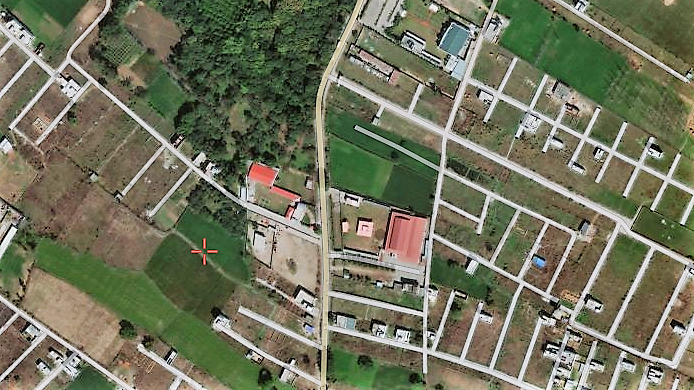
\includegraphics[width=0.25\textwidth]{./pictures/fimg8.png} & 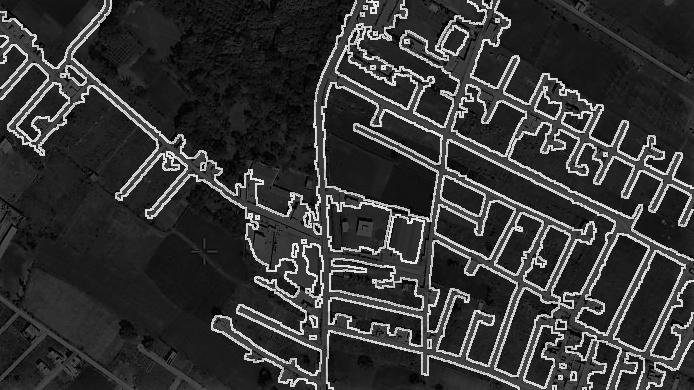
\includegraphics[width=0.25\textwidth]{./pictures/fimg8.png_final_img.jpg} & 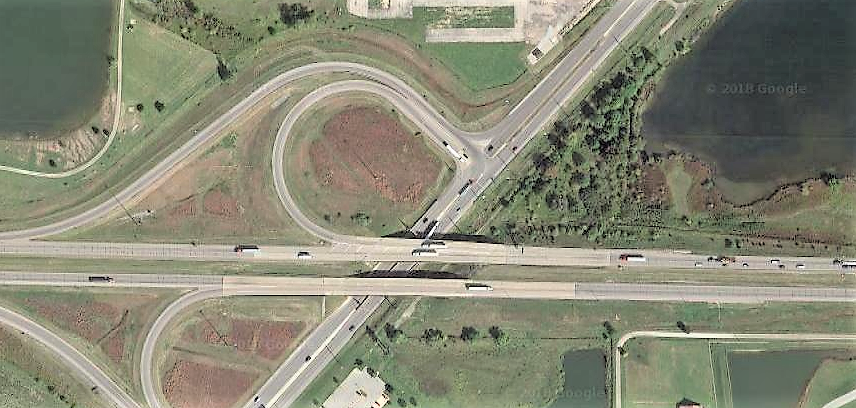
\includegraphics[width=0.25\textwidth]{./pictures/fimg12.png} & 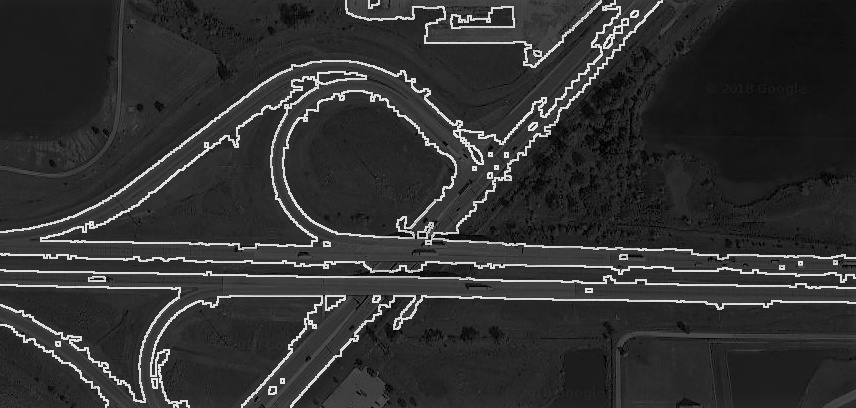
\includegraphics[width=0.25\textwidth]{./pictures/fimg12.png_final_img.jpg}\\
 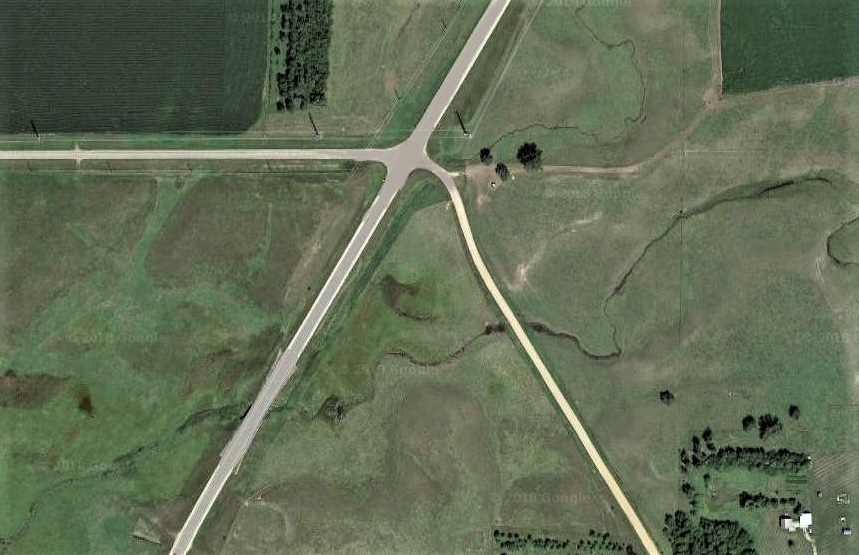
\includegraphics[width=0.25\textwidth]{./pictures/fimg10.png} & 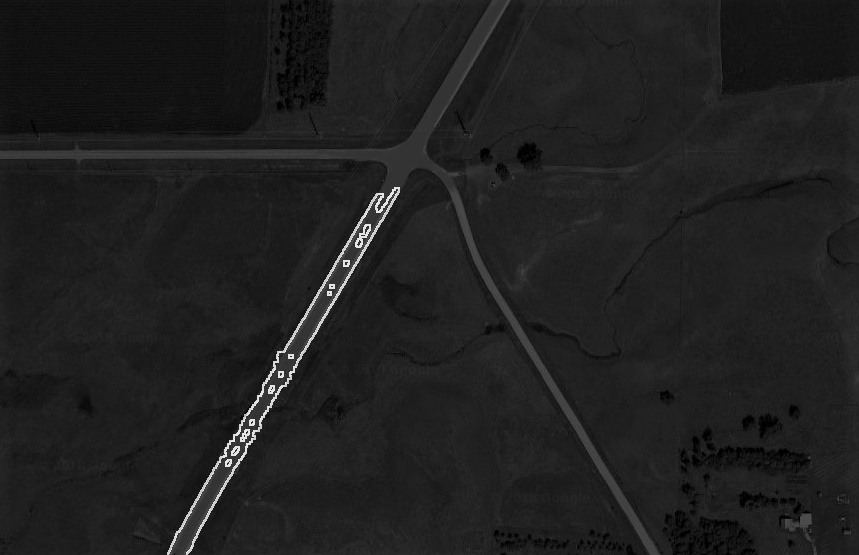
\includegraphics[width=0.25\textwidth]{./pictures/fimg10.png_final_img.jpg} & 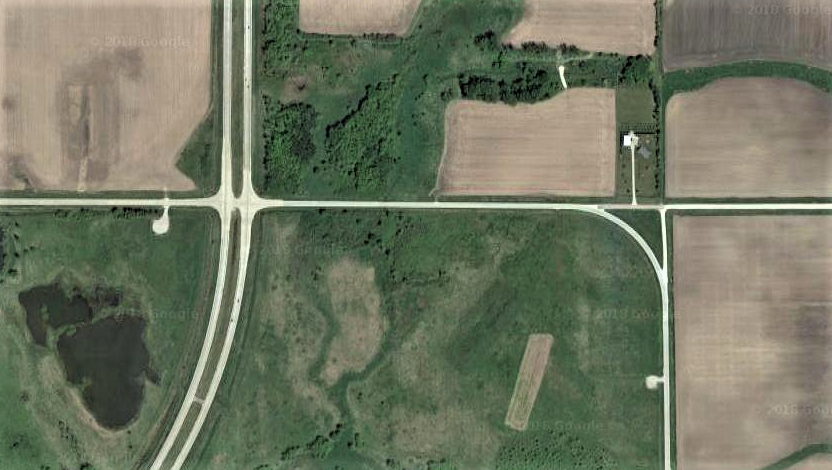
\includegraphics[width=0.25\textwidth]{./pictures/fimg11.png} & 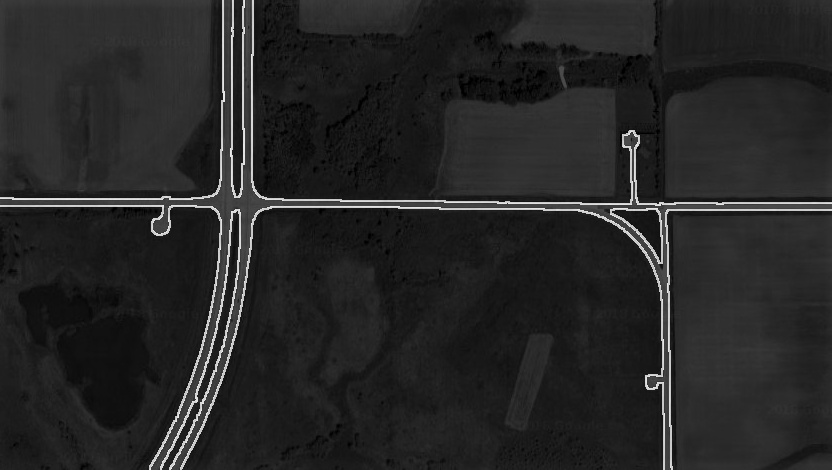
\includegraphics[width=0.25\textwidth]{./pictures/fimg11.png_final_img.jpg}\\ 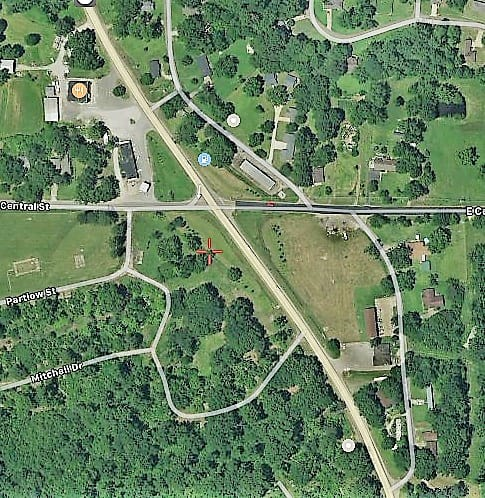
\includegraphics[width=0.25\textwidth]{./pictures/fimg9.jpeg} & 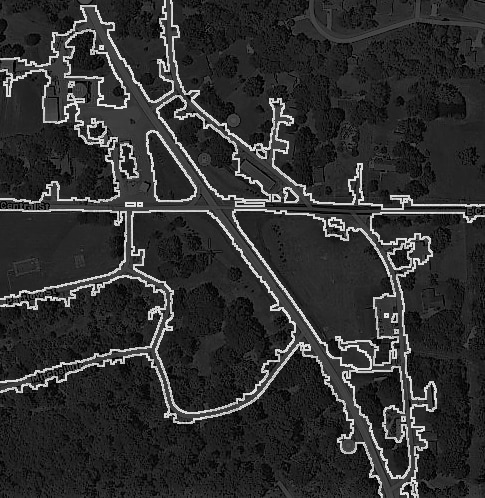
\includegraphics[width=0.25\textwidth]{./pictures/fimg9.jpeg_final_img.jpg} & 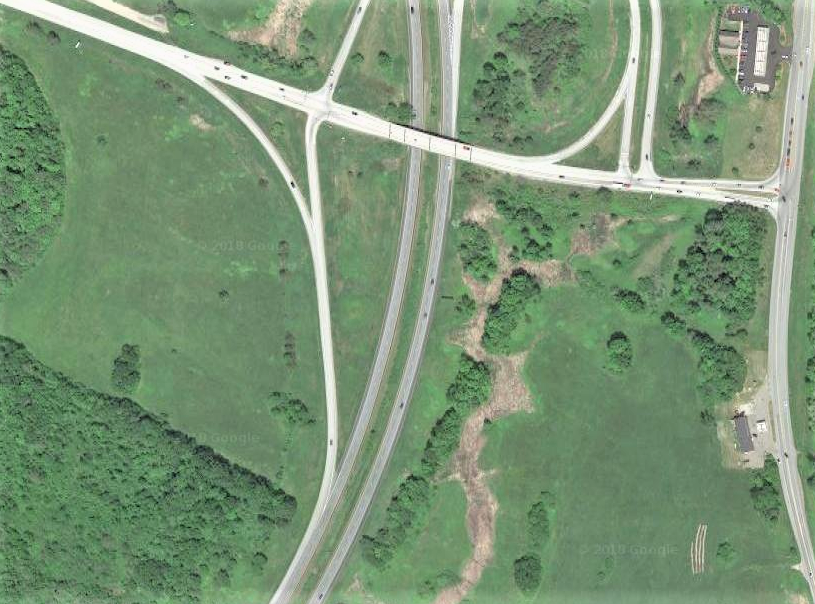
\includegraphics[width=0.25\textwidth]{./pictures/fimg14.png} & 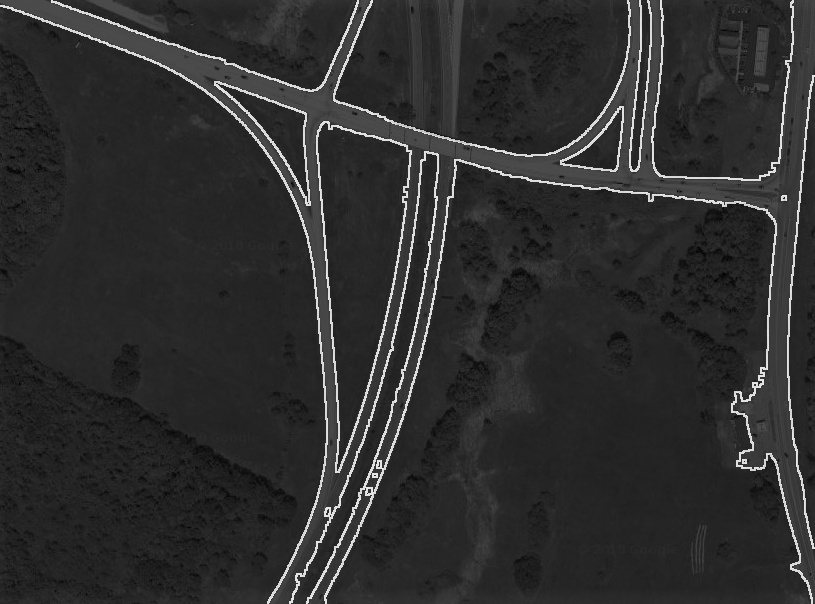
\includegraphics[width=0.25\textwidth]{./pictures/fimg14.png_final_img.jpg}
\end{tabular}
 \newgeometry{
 a4paper,
 total={170mm,257mm},
 left=40mm,
 top=25mm,
 bottom=25mm,
 right=25mm
 }
\section{Results and Discussion}
Using basic image processing techniques like : grayscale conversion, contrast stretching, thresholding, filtering, dilation, morphological enhancement, closing and edge detection techniques on available satellite images we can accurately highlight the roads present in the images (with acceptable precision) depending on image availability provided is high resolution.\\
Following example image signifies the how roads highlighted show intricate details of the street structure.
\begin{center}
\begin{tabular}{ c c}
 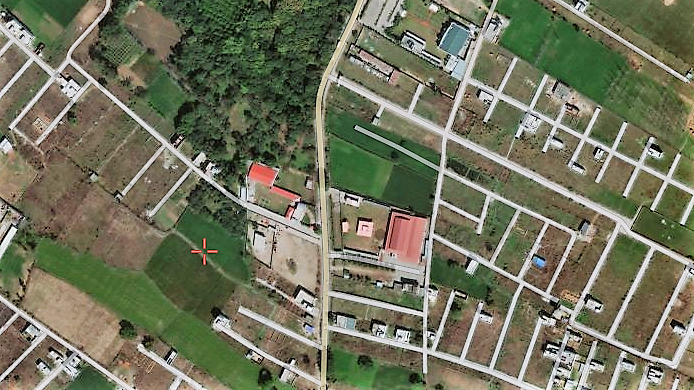
\includegraphics[width=0.5\textwidth]{./pictures/fimg8.png} & 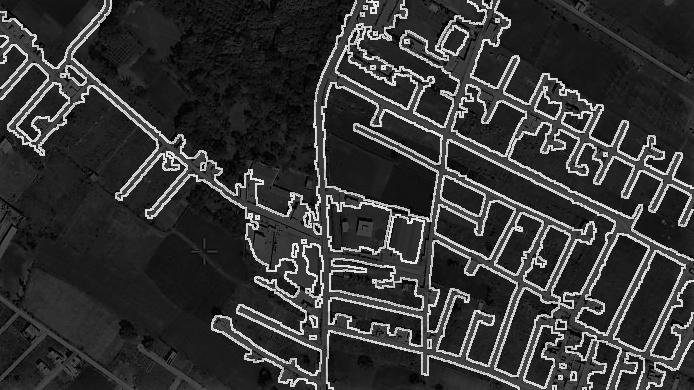
\includegraphics[width=0.5\textwidth]{./pictures/fimg8.png_final_img.jpg}
\end{tabular}
\end{center}
Although it works fairly accurately in above images still it has several limitation in some cases as shown below due to less resolution images and due to bad quality of colour saturation causing defect in the intensity.
\begin{center}
\begin{tabular}{ c c}
 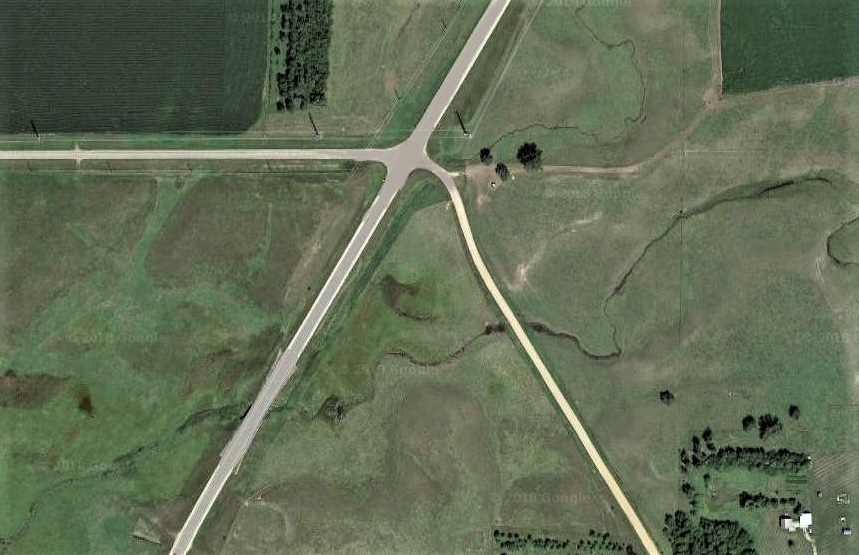
\includegraphics[width=0.5\textwidth]{./pictures/fimg10.png} & 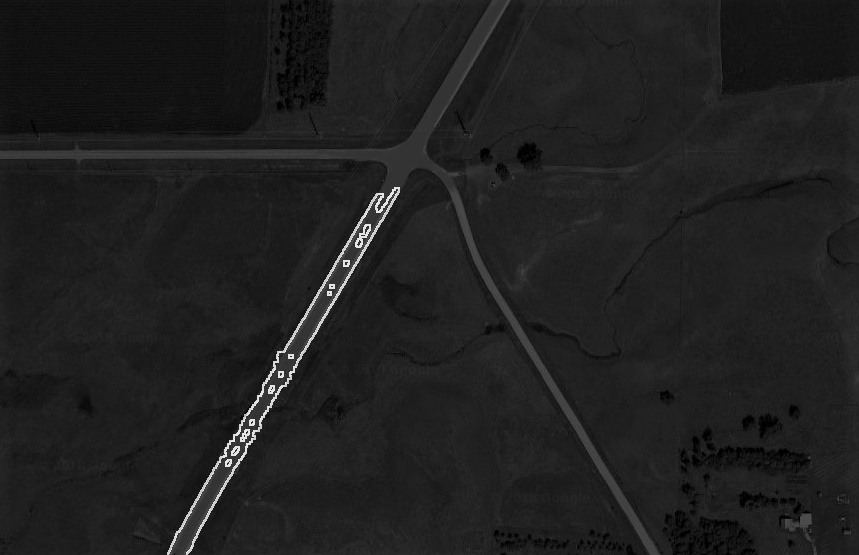
\includegraphics[width=0.5\textwidth]{./pictures/fimg10.png_final_img.jpg}
\end{tabular}
\end{center}

\section{Conclusion}
Through this paper we conclude that using even the most basic techniques of image processing most intricate tasks like highlighting roads from satellite images can be easily done with fairly accurate results in most cases.
It cannot be refused that a better road extraction algorithm may exist but this paper reflects use of only primary operations and concepts of image processing to implement a useful application.
All the operation used in this project were all learned in the IVP course and as much as possible all of them are coded from scratch with contribution from each team member in the process.
\newpage
\section{Contribution}
\begin{itemize}
  \item \textbf{Pradhuman Singh: } Arrange research paper, creation of latex doc, helped in coding.
  \item \textbf{Shyam Tayal: } Creation of Latex Doc, drawing flowchart, fix bugs in code.
  \item \textbf{Abhijeet Sonkar: } Arrange research paper, help in code and drawing flow chart.
  \item \textbf{Avneesh Kumar: } Creation of Latex Doc, wrote code for project.
  \item \textbf{Arvind Uikey: } Arrange research paper, creation of latex doc, arranging images.
  \item \textbf{Hitika Rajesh Kumar: } Creation of Latex Doc, helped in coding, arranged images.
\end{itemize}

\newpage

\begin{thebibliography}{9}
\bibitem{paper}
{J. Dai; T. Zhu; Y. Wang; R. Ma and X. Fang}, \emph{Road Extraction From High-Resolution Satellite Images Based on Multiple Descriptors in IEEE Journal of Selected Topics in Applied Earth Observations and Remote Sensing}
\\ [0.01in]
\bibitem{paper}
Xin, J.; Zhang, X.; Zhang, Z.; Fang, W. \emph{Road Extraction of High-Resolution Remote Sensing
Images Derived from DenseUNet}
\\ [0.01in]
\bibitem{book}
Gonzalez, R. C., Woods, R. E. (2008) \emph{Digital image processing}, Prentice Hall.
\\ [0.01in]
\bibitem{paper}Xiangyun Hu and Vincent Tao, \emph{Automatic Extraction of Main Road Center lines from High Resolution Satellite Imagery Using Hierarchical Grouping, Photogrammetric Engineering and Remote Sensing, Vol. 73, No. 9, pp. 1049- 1056, 2007}
\\ [0.01in]
\bibitem{paper} Anil and NataRajan, \emph{Automatic Road Extraction from High Resolution Imagery Based on Statistical Region Merging and Skeletonization, International Journal of Engineering Science and Technology Vol. 2, No.3, pp.165-171, 2010}

\end{thebibliography}
\end{document}
